\chapter[MoM Introduction]{Introduction to the Method of Moments Using
  Electrostatics \label{chap:momIntro}} 

%\setcounter{page}{1}

\renewcommand{\thefootnote}{\fnsymbol{footnote}}
\footnotetext[2]{EE 351.  Lecture notes by John Schneider.  {\tt
mom-intro.tex}}

\section{Introduction}

The method of moments (MoM) provides a way to solve integral equations
in which an unknown function appears in the integrand.  Many problems
in electromagnetics can be cast in the form of such integral
equations.  Here the method of moments will be used to solve problems
in electrostatics.  However, the concepts used to formulate the
solution carry over to time harmonic problems too (even though the
governing integral equations are different).  As will be shown, MoM
relies upon the expansion of the unknown function in a set of basis
functions.  The basis functions are known, and hence can be
integrated, but the coefficients of the basis function are unknown.
Nevertheless, one can solve for these coefficients.  The integral
equations which govern the potential about a collection of static
charge is relatively straightforward and hence electrostatics will be
used to introduce MoM.

\section{Electrostatics}

Before embarking on MoM, we review electrostatics and show how one can
solve for unknown charges given information about the potential about
the charges.  The potential about a point charge $Q$ is given by
\begin{equation}
  V(\rvec) = \frac{Q}{4 \pi \epsilon_0|\rvec-\rvec'|} \label{eq:pointCharge}
\end{equation}
where $V$ is the voltage, $\rvec$ is the observation point, and $\rvec'$
gives the location of the charge (i.e., the source point).  Assume, as
depicted in Fig.\ \ref{fig:singleCharge}, a single unknown charge $Q_1$
is located at $\rvec_1'$.  Although the charge is unknown, assume the
voltage at location $\rvec_1$ is known, i.e., $V(\rvec_1)=V_1$.  Given
this information, \refeq{eq:pointCharge} can be solved for the charge
\begin{equation}
  Q_1 =  4 \pi \epsilon_0|\rvec_1-\rvec_1'| V(\rvec_1) 
      =  4 \pi \epsilon_0R_{11} V(\rvec_1) 
\end{equation}
where $R_{11} = |\rvec_1-\rvec_1'|$.  Thus, to find the charge we must
know the potential at a point, where the potential was observed, and
where the charge is located.  It is important to note that we needed
to know the potential at a single point to solve for the charge.
However, once that charge is known, the potential is known throughout
space via \refeq{eq:pointCharge}.
\begin{figure}
  \begin{center}
  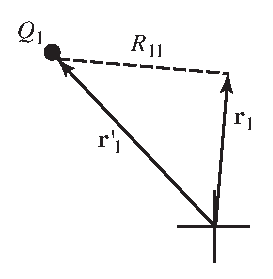
\epsfig{width=2.in,file=Figures/Mom-intro/singleCharge.eps}
  \end{center}
  \caption{The potential observed at $\rvec_1$ is due to a point charge
    $Q_1$ located at $\rvec_1'$.}
  \label{fig:singleCharge}
\end{figure}

Now consider the situation shown in Fig.\ \ref{fig:doubleCharge} where
there are two unknown charges, $Q_1$ and $Q_2$, located at known
positions $\rvec_1'$ and $\rvec_2'$, respectively.
\begin{figure}
  \begin{center}
  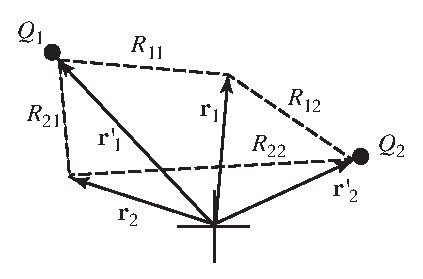
\epsfig{width=3.25in,file=Figures/Mom-intro/doubleCharge.eps}
  \end{center}
  \caption{Two unknown point charges located at known positions.  The
    voltage is known at locations $\rvec_1$ and $\rvec_2$.}
  \label{fig:doubleCharge}
\end{figure}
In this case the potential at an arbitrary point in space would be
given by
\begin{equation}
  V(\rvec) = \frac{Q_1}{4 \pi \epsilon_0|\rvec-\rvec_1'|} 
        + \frac{Q_2}{4 \pi \epsilon_0|\rvec-\rvec_2'|}.
  \label{eq:twoCharges}
\end{equation}
Since there are two unknowns, one cannot solve for the charges by
observing the potential at a single point.  However, if the voltage is
known at two points, $\rvec_1$ and $\rvec_2$, it may be possible to solve
for the two charges.  The relevant equations are
\begin{eqnarray}
  V(\rvec_1) \,=\, V_1 \!&=& \frac{Q_1}{4 \pi \epsilon_0R_{11}} 
              + \frac{Q_2}{4 \pi \epsilon_0R_{12}}, \\
  V(\rvec_2) \,=\, V_2 \!&=& \frac{Q_1}{4 \pi \epsilon_0R_{21}} 
              + \frac{Q_2}{4 \pi \epsilon_0R_{22}},
\end{eqnarray}
where $R_{mn}=|\rvec_m-\rvec_n'|$ is the distance between the $m$th
observation point and the $n$th charge, and $V_m$ is the voltage at the
$m$th observation point.  Written in matrix form this becomes
\begin{eqnarray}
  \left[
   \begin{array}{c}
      V_1 \\
      V_2 
   \end{array}
  \right] &=& 
  \frac{1}{4\pi\epsilon_0}
  \left[
    \begin{array}{cc}
      \frac{1}{R_{11}} & \frac{1}{R_{12}} \\
      \frac{1}{R_{21}} & \frac{1}{R_{22}}
    \end{array}
  \right]
  \left[
    \begin{array}{c}
      Q_1 \\
      Q_2 
    \end{array}
  \right] \\
  \left[V_m\right] &=& \left[Z_{mn}\right] \left[Q_n\right]
\end{eqnarray}
where the elements of the $Z_{mn}$ matrix are given by
$1/(4\pi\epsilon_0 R_{mn})$.

Thus the unknown charges can be obtained from
\begin{equation}
  \left[Q_n\right] = \left[Z_{mn}\right]^{-1} \left[V_m\right].
  \label{eq:qnVector}
\end{equation}
This equation can be generalized to any number of unknown charges.  In
order to solve for the charges one needs as many equations are there
are unknowns, i.e., one must know the voltage at as many discrete
locations as there are charges.  Additionally, the $Z_{mn}$
matrix must be invertible.  This places some restriction on the
observations points.  Consider the scenario shown in
Fig.\ \ref{fig:singularZ} where the observation points lie in a plane
half way between $Q_1$ and $Q_2$ and which is perpendicular to the line
passing through $Q_1$ and $Q_2$.  In this case $R_{11}=R_{12}$ and 
$R_{21}=R_{22}$.  Therefore the rows of the $Z_{mn}$ matrix are not
independent and the matrix cannot be inverted.  
\begin{figure}
  \begin{center}
  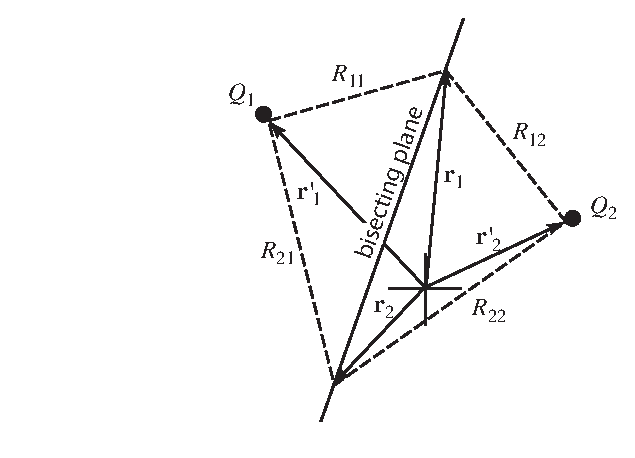
\epsfig{width=3.in,file=Figures/Mom-intro/bisectingDouble.eps}
  \end{center}
  \caption{The selection of observations points is not arbitrary.  In
    the arrangement shown above, $R_{11}=R_{12}$ and $R_{21}=R_{22}$
    which causes the $Z_{mn}$ matrix to be singular.}
  \label{fig:singularZ}
\end{figure}

As was the case for the single charge, once all the charges in the
system are known, the potential can be found at an arbitrary location.
In many ways the method of moments is simply an extension of this sort
of solving for the charge in a system.  In order to solve for charge,
the potential has to be known over some region of space.  Once the
charge is known, the potential can be calculated anywhere.

\section{Continuous Distribution of Charge}

When the charge is distributed continuously over space it is described
by either a surface or a volume charge-density function.  The point
charge $Q$ is replaced by either $\rho_s(\rvec')ds'$ or
$\rho_v(\rvec')dv'$ where $\rho_s(\rvec')$ is a surface charge-density
function (C/m$^2$), $ds'$ is an incremental area (m$^2$),
$\rho_v(\rvec')$ is a volume charge-density function (C/m$^3$), and
$dv'$ is an incremental volume (m$^3$).  Instead of using a discrete
sum of contributions from discrete charges, when there is a continuous
distribution of charge one must use a continuous sum, i.e., an
integral, to find the voltage at an arbitrary point.  If a system has
discrete charges, surface charge, and volume charge, the voltage at an
arbitrary point would be given by
\begin{equation}
  V(\rvec) =
  \sum_{n=1}^{N}\frac{Q_n}{4\pi\epsilon_0|\rvec-\rvec_n'|} +
  \iint_{S}\frac{\rho_s(\rvec')ds'}{4\pi\epsilon_0|\rvec-\rvec'|} +
  \iiint_{V}\frac{\rho_v(\rvec')dv'}{4\pi\epsilon_0|\rvec-\rvec'|}.
  \label{eq:potentialGeneral}
\end{equation}
The goal is to be able to find the charge distribution given the
voltage over some region of space.

As shown in Fig.\ \ref{fig:singlePlate}, consider a conducting square
plate with unit area on which the potential is 1 V.  What is the
potential at an arbitrary point about this plate?  One cannot answer
that question until the charge distribution over the plate is known.
\begin{figure}
  \begin{center}
  \epsfig{width=3.in,file=Figures/Mom-intro/singlePlate.eps}
  \end{center}
  \caption{A conducting square plate with unit area on which the
    potential is 1 V.  The charge density is not given.  To find the
    potential at an arbitrary point the charge density must be found.}
  \label{fig:singlePlate}
\end{figure}
For this case, using an observation point on the plate,
\refeq{eq:potentialGeneral} becomes
\begin{equation}
  V(\rvec) = 1 = 
  \left.
    \int_{x'=0}^1\int_{y'=0}^1
  \frac{\rho_s(\rvec')dx' dy'}{4\pi\epsilon_0|\rvec-\rvec'|}
  \right|_{\rvec\in{\mbox{plate}}}.
  \label{eq:vPlate}
\end{equation}
The observation and source points can be written
$\rvec=x\unitvec{x}+y\unitvec{y}$ and
$\rvec'=x'\unitvec{x}+y'\unitvec{y}$, respectively, so that
$|\rvec-\rvec'|=((x-x')^2+(y-y')^2)^{1/2}$.  

The function $\rho_s(\rvec')$ is unknown and appears within the
integrand.  To solve for it, the charge density is approximated by a
sum of known basis functions with constant, but unknown, coefficients, i.e., 
\begin{equation}
  \rho_s(\rvec') \approx \sum_{n=1}^N a_n g_n(\rvec'),
\end{equation}
where $a_n$ are the coefficients and $g_n$ are the basis functions.
Using this expression for the charge density in \refeq{eq:vPlate} and
interchanging the order of differentiation and summation yields
\begin{equation}
 1 = 
\sum_{n=1}^N a_n 
  \left.
    \int_{x'=0}^1\int_{y'=0}^1
  \frac{g_n(\rvec')dx' dy'}{4\pi\epsilon_0|\rvec-\rvec'|}
  \right|_{\rvec\in{\mbox{plate}}}.
  \label{eq:vPlateBasis}
\end{equation}
Since the basis functions are known, these integrals can be calculated
(although they may have to be calculated numerically).  At this point
it appears there is one equation and $N$ unknowns (the $N$
coefficients $a_n$).  However, the observation point has not been
specified and thus it is possible to generate $N$ unique equations
from \refeq{eq:vPlateBasis}.

\section{Pulse Basis Functions with Point Matching
\label{sec:pulsePoint}}

There are essentially an infinite variety of basis functions one
can use to model the charge distribution.  There are also various
schemes for determining the unknown coefficients.  Here we will use
what is arguably the simplest approach: pulse basis functions with
point matching.

Pulse basis functions have unit magnitude over some domain and are
zero everywhere else.  For the plate problem shown in
Fig.\ \ref{fig:singlePlate}, we will use square basis functions that
have a width of $\Delta$.  Assume, as shown in
Fig.\ \ref{fig:basisFunctions}, there are 100 total basis functions
used to model the charge on the plate.  There are 10 basis
functions, or cells, per side.
\begin{figure}
  \begin{center}
  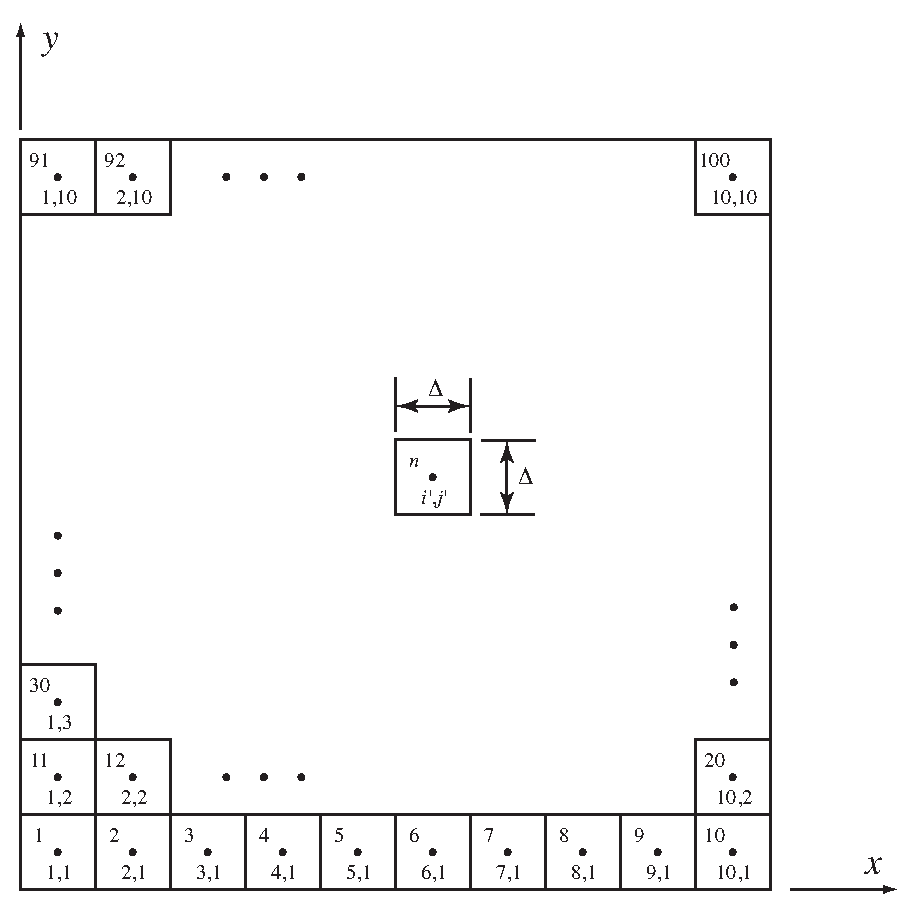
\epsfig{width=4.5in,file=Figures/Mom-intro/basisFunctionsPlate.eps}
  \end{center} \caption{Discretization of a plate into 100 square
  basis functions, each with width $\Delta$.  Shown within each basis
  function, or cell, are three numbers.  The upper left number
  corresponds to the basis function number (the ``global number'').
  Two indices are also given which are the ``positional indices.''
  The first of these, the $i'$ index, indicates the displacement in
  the $x$ direction while the second, the $j'$ index, indicates
  displacement in the $y$ direction.  The center of the cell is
  indicated by a dot.}  \label{fig:basisFunctions}
\end{figure}
Assuming unit length for the sides of the square plate, the width of
the individual cells is $\Delta = 1/10$.  As shown in Fig.\
\ref{fig:basisFunctions}, each cell is assigned a ``global number''
$n$, here ranging between 1 and 100.  Additionally, each cell also has
two positional indices associated with it.  The first, or $i'$ index,
indicates the displacement in the $x$ direction while the second, or
$j'$ index, indicates displacement in the $y$ direction (the reason
for using the primes on the indices will become apparent later).  One
can obtain the global number $n$ from the $i'$ and $j'$ indices via
\begin{equation}
  n = 10(j'-1) + i'.
\end{equation}
Conversely, the $i'$ and $j'$ indices can be obtained from the global
index using the following two equations
\begin{eqnarray}
  j' &=& \mbox{int}((n-1)/10) + 1, \label{eq:jFromGlobal} \\
  i' &=& m - 10(j'-1), \label{eq:iFromGlobal}
\end{eqnarray}
where int() indicates the integer portion of the argument.  
The center
of the $n$th cell is given by
\begin{equation}
  \rvec_n = (i'-1/2)\Delta \unitvec{x} +  (j'-1/2)\Delta \unitvec{y}.
  \label{eq:centers}
\end{equation}
The pulse basis functions are defined by
\begin{equation}
  p_n(x',y',z') = \left\{
  \begin{array}{l}
    1\quad \mbox{if} \quad\left\{
      \begin{array}{l}
        (i'-1)\Delta \leq x' \leq i'\Delta \\
        (j'-1)\Delta \leq y' \leq j'\Delta \\
        z=0
      \end{array}\right. \\
    0\quad \mbox{otherwise}
  \end{array}\right.
  \label{eq:pulseDetails}
\end{equation}
or, said more simply, the basis function is unity if the point is
within the cell and zero otherwise.  This expression for
$p_n(x',y',z')$ is used for the generic basis function $g_n(\rvec')$ in
\refeq{eq:vPlateBasis}.  This yields
\begin{equation}
 1 = 
\sum_{n=1}^N a_n 
  \left.
    \int_{x'=(i'-1)\Delta}^{i'\Delta}\int_{y'=(j'-1)\Delta}^{j'\Delta}
  \frac{dx'dy'}{4\pi\epsilon_0|\rvec-(x'\unitvec{x}+y'\unitvec{y})|}
  \right|_{\rvec\in{\mbox{plate}}}.
  \label{eq:vPlateBasisI}
\end{equation}
In order to solve for the unknown coefficients $a_n$, we use a
point-matching scheme which is to say that \refeq{eq:vPlateBasisI}
will be satisfied at discrete observation points.  We take these
observation points to be the centers of the cells.  Since there are
100 cells, this yields 100 equations, each with 100 unknowns.  For the
observation points, a global index $m$ will be used, which has
corresponding positional indices $i$ and $j$.  Thus, the observation
points are given by \refeq{eq:centers} with $n$ replaced by $m$, $i'$
replaced with $i$, and $j'$ replaced with $j$.  Using such an
observation point in
\refeq{eq:vPlateBasisI} yields
\begin{equation}
1 = 
\sum_{n=1}^N a_n 
  \int_{x'=(i'-1)\Delta}^{i'\Delta}\int_{y'=(j'-1)\Delta}^{j'\Delta}
  \frac{dx'dy'}{4\pi\epsilon_0
                \left|\left(\left(i-\frac{1}{2}\right)\Delta\unitvec{x}
                +\left(j-\frac{1}{2}\right)\Delta\unitvec{y}\right)
                 -(x'\unitvec{x}+y'\unitvec{y})\right|}.
  \label{eq:vPlateBasisII}
\end{equation}
Note that the left-hand side represents the voltage at the observation
point $\rvec_m$ but in this case the voltage is always unity, i.e.,
$V(\rvec_m)=V_m=1$.

The double integral in \refeq{eq:vPlateBasisII} yields the potential
at observation point $\rvec_m$ due to basis function $n$.  (Keep in mind
that $m$ dictates the values of $i$ and $j$ while $n$ dictates the
value of $i'$ and $j'$.)  These integrals are similar to the $Z_{mn}$
terms described in the point-charge problem which gave the potential
at observation point $m$ due to charge $n$.  Thus these integrals are
also labeled $Z_{mn}$:
\begin{equation}
Z_{mn} = 
  \int_{x'=(i'-1)\Delta}^{i'\Delta}\int_{y'=(j'-1)\Delta}^{j'\Delta}
  \frac{dx'dy'}{4\pi\epsilon_0
                \left|\left(\left(i-\frac{1}{2}\right)\Delta\unitvec{x}
                +\left(j-\frac{1}{2}\right)\Delta\unitvec{y}\right)
                 -(x'\unitvec{x}+y'\unitvec{y})\right|}.
  \label{eq:zmn}
\end{equation}
In order to solve the system of equations, one must find $Z_{mn}$ for
each combination of observation point and source point (i.e., each
combination of $m$ and $n$).  For the square basis functions described
here, these integrals can be done exactly.  However, there are some
approximations which can be used which greatly simplify the problem.

The pulse basis functions are generally assumed to be small enough so
that the integrand does not change significantly over the limits of
integration.  Thus, it is typically good enough to assume that $x'$
and $y'$ are fixed at the center of the $n$th cell.  In this way $Z_{mn}$
can be approximated as
\begin{eqnarray}
Z_{mn} &\approx&
  \frac{1}{4\pi\epsilon_0 |\rvec_m-\rvec_n|}
  \int_{x'=(i'-1)\Delta}^{i'\Delta}\int_{y'=(j'-1)\Delta}^{j'\Delta}
  dx'dy', \nonumber\\
 &=&  \frac{\Delta^2}{4\pi\epsilon_0|\rvec_m-\rvec_n|} \\
 &=&  \frac{\Delta^2}{4\pi\epsilon_0
            |(x_m-x_n)\unitvec{x}-(y_m-y_n)\unitvec{y}|}.
  \label{eq:zmnApprox}
\end{eqnarray}
The distance $|\rvec_m-\rvec_n|$ is the distance between the center of the
$m$th cell and the $n$th cell.  Breaking this into $x$ and $y$
components yields
\begin{eqnarray}
  x_m-x_n \!&=&\! (i-1/2)\Delta - (i'-1/2)\Delta = (i-i')\Delta, \\
  y_m-y_n \!&=&\! (j-1/2)\Delta - (j'-1/2)\Delta = (j-j')\Delta.
\end{eqnarray}
Thus the distance between these two points is
\begin{equation}
  |\rvec_m-\rvec_n| = \left((i-i')^2 + (j-j')^2\right)^{1/2}\Delta.
\end{equation}
Plugging this into \refeq{eq:zmnApprox} yields
\begin{equation}
  Z_{mn} =  \frac{1}{4\pi\epsilon_0}
            \frac{\Delta}{\left((i-i')^2 + (j-j')^2\right)^{1/2}}.
  \label{eq:zmnApproxI}
\end{equation}
Note that if the observation point and the source point are
interchanged, the results is the same: $Z_{mn}$ only depends on the
distance between the points $\rvec_m$ and $\rvec_n$ and it does not matter which
one we call the source point and which we call the observation point.
Therefore $Z_{mn}$ equals $Z_{nm}$.

The approximation used in \refeq{eq:zmnApprox} is equivalent to
assuming that instead of having the charge uniformly distributed over
the basis function (i.e., uniformly distributed over the $n$th cell),
all the charge is concentrated at a point at the center of the $n$th
cell.  Since the basis function has unit charge density over an area
of $\Delta^2$, the charge associated with the cell (ignoring for the
moment the $a_n$ coefficient) is simply $\Delta^2$ and
$\Delta^2/(4\pi\epsilon_0|\rvec_m-\rvec_n|)$ is the potential associated
with this charge when observed at point $\rvec_m$.

However, this approximation will not work when the observation point
is at the center of the $n$th cell, i.e., when $m=n$.  For $Z_{mm}$
one must account for the distribution of charge over the surface of
the cell (otherwise the potential appears infinite at the center of a
point charge).  When $m=n$ one can always do a variable substitution
to write the integral as
\begin{equation}
  Z_{mm} = 
  \int_{x'=-\Delta/2}^{\Delta/2}\int_{y'=-\Delta/2}^{\Delta/2}
  \frac{dx'dy'}{4\pi\epsilon_0
    \left(x'^2 + y'^2\right)^{1/2}} =
   \frac{2\Delta}{4\pi\epsilon_0}
   \ln\!\left(\frac{\sqrt{2}+1}{\sqrt{2}-1}\right).
   \label{eq:zmm}
\end{equation}
The expression shown on the right is exact.

We can now cast the solution to the problem in the same form as the
previous section.  The charge is (or, more properly, the basis-function
coefficients are) given by
\begin{equation}
  [a_n] = [Z_{mn}]^{-1}[V_m],
\end{equation}
where the $Z_{mn}$ elements are given by \refeq{eq:zmnApproxI} for the
off-diagonal terms and by \refeq{eq:zmm} for the diagonal terms.

\section{Solving for the Charge on a Plate Using Matlab}

In this section we wish to solve for the charge distribution on the
plate which was described in the previous section.  The solution
requires the inversion of a $100\times 100$ matrix which can be
implemented using various computer languages or programs.  Matlab is
especially well suited to matrix and vector manipulation so it will be
used here.  However, one should keep in mind that Matlab was
originally just a front-end to the LINPACK library of linear algebra
routines that one can download for free (these routines were
originally written in FORTRAN but C versions are also available).

The generation of the voltage vector $V_m$ is rather trivial. Instead
of fixing the voltage of the plate at 1 V, we allow the user to
specify the voltage.  Additionally, instead of fixing the number of
cells per side of the plate at 10, we allow the user to specify an
arbitrary number of cells.  A function to accomplish this is shown in
Program \ref{pro:vm}.  This function uses the built-in Matlab function
{\tt repmat} to repeat the voltage term the necessary number of times.
{\tt repmat} copies its argument to memory the specified number of
times and typically is faster than other ways of creating an array
with repeated entries (such as creating an array of ones and then
multiplying the unity array elements by the desired term).  Note that
the factor of $4\pi\epsilon_0$ has been moved from the denominator of
the $Z_{mn}$ elements to the numerator of the voltage elements.
\begin{program}
Matlab function to generate the voltage vector $V_m$.  The
vector includes the factor $4\pi\epsilon_0$. \label{pro:vm}
\codemiddle
\begin{lstlisting}[language=Matlab]
function vm = makeVmPlate(voltage,numPerSide)
% makeVmPlate  Make the voltage vector for a square plate.
%
% vm=makeVmPlate(voltage,numPerSide) Returns the vector Vm for
%    a square plate with a total of numPerSide^2 cells.  The
%    voltage is specified by the first argument.  The factor of
%    4*pi*epsilon_0 is included in the voltage vector (rather
%    than in the Zmn matrix).

numPerPlate = numPerSide^2;  % total number of cells on plate

vm = repmat(voltage * 4.0 * pi * 8.854e-12,numPerPlate,1);

return;
\end{lstlisting}
\end{program}

Next, let us define a Matlab function {\tt m2ij} which returns the
positional indices $i$ and $j$ when given the global number $m$.  A
suitable function is shown in Program \ref{pro:m2ij}.
\begin{program}
Matlab function to convert from global index $m$ to position
indices $i$ and $j$. \label{pro:m2ij}
\codemiddle
\begin{lstlisting}[language=Matlab]
function [i, j] = m2ij(m,numPerSide)
% M2IJ Convert the global index m to the positional
%   indices i and j.
%
%   [i, j] = m2ij(m,numPerSide) where m is the global index
%   and numPerSide is the number of elements along one side of
%   the plate.

j = floor((m-1)/numPerSide) + 1;

i = m - numPerSide*(j-1);

return;
\end{lstlisting}
\end{program}
This function takes two arguments.  The first is the global index and
the second is the number of cells per side of the plate.  The function
returns the two scalar positional indices.  Note that this same
function pertains to conversion of the global index $n$ to the
positional indices $i'$ and $j'$.  One merely has to give ``$n$'' as
the first argument rather than ``$m$.''

Program \ref{pro:zmn} shows a Matlab function which is suitable for
creating the $Z_{mn}$ matrix.  Again, the number of cells per side of
the plate is specified as an argument (the single argument passed to
the function).  The ``self term'' is calculated in line 16 and this
term is put on the diagonal of the matrix using the commands {\tt
repmat} and {\tt diag}.  The off-diagonal terms are calculated in the
nested loops starting at line 20.  As mentioned in connection with the
generation of the voltage vector, the factor of $4\pi\epsilon_0$ does
not appear in this function since it is now included in the voltage
vector.  The outer loop starting at line 20 represents the observation
point $m$.  The inner loop starting at line 22 represents the basis
function (or source term) $n$.  The index for the inner loop starts
with a value of $m+1$.  This serves to fill the upper half of the
$Z_{mn}$ matrix.  The statement in line 25 exploits the symmetry that
$Z_{nm}=Z_{mn}$ to ensure the lower half of the matrix is filled.  The
function {\tt m2ij} is used in lines 21 and 23 to convert the global
indices $m$ and $n$ to the pairs of positional indices $(i,j)$ and
$(i',j')$, respectively.
\begin{program}
Matlab function to generate the $Z_{mn}$ matrix. \label{pro:zmn}
\codemiddle
\begin{lstlisting}[language=Matlab]
function zmn = makeZmnPlate(numPerSide)
% makeZmnPlate  Make the Zmn matrix for a square plate.
%
% zmn = makeZmnPlate(numPerSide) Creates the Zmn matrix for a
%    square plate where each basis function is a square pulse.
%    The area of the basis functions is (1/numPerSide)^2, i.e.,
%    the plate is assumed to have unit area and is divided into
%    numPerSide^2 square cells.

del  = 1/numPerSide;        % length of the side of a cell
del2 = del^2;               % area of a cell
numPerPlate = numPerSide^2; % total number of elements on a plate

% Place self term (exact Zmm term) along diagonal of matrix.
zmn = diag(...
    repmat(2.0*del*log((sqrt(2)+1)/(sqrt(2)-1)),numPerPlate,1)...
    );

% Calculate the off-diagonal terms.
for m=1:numPerPlate
  [i j] = m2ij(m,numPerSide);       % observation point
  for n=m+1:numPerPlate
    [ip jp]  = m2ij(n,numPerSide);  % source point
    zmn(m,n) = del/sqrt((i-ip)^2 + (j-jp)^2);
    zmn(n,m) = zmn(m,n);  % exploit symmetry to fill lower half
  end
end

return;
\end{lstlisting}
\end{program}

Given these three functions, just a few more lines of Matlab code are
required to obtain the coefficients of the basis functions.  A sample
session is shown in Program \ref{pro:plateSession}.  The number of
cells per side of the plate is set in line 2.  The voltage vector is
generated in line 5.  The $Z_{mn}$ matrix is generated in line 8 and
the basis-function coefficients are obtained in line 11.  Given
these coefficients the total charge on the plate can be calculated by
summing the charge on each basis function, i.e., 
\begin{equation}
  Q_{\text{total}} = \sum_{n=1}^{100} a_n \left(\frac{1}{10}\right)^2.
\end{equation}
The factor of 1/10 is the width of a single cell so that this value
squared is the area of the cell. 
\begin{program}
Matlab session to calculate and display the charge on a
square plate. \label{pro:plateSession}
\codemiddle
\begin{lstlisting}[language=Matlab]
% Set the number of cells per side of the plate.
numPerSide = 10;

% Generate voltage vector assuming unit voltage on plate.
vm  = makeVmPlate(1,numPerSide);

% Calculate the Zmn matrix.
zmn = makeZmnPlate(numPerSide);

% Solve for the basis-function coefficients.
an = zmn \ vm;

% Calculate the total charge on plate.
del=1.0/numPerSide;  %%% width of a cell
charge = sum(an)*del^2;

%%%
% Plot coefficients of all basis functions.
figure(1)
plot(an)      %%% show as a connected curve
hold
plot(an,'.')  %%% show the discrete values
title(...
  strcat('Charge vs. Basis Function Number, \Delta=1/',...
          num2str(numPerSide)));
xlabel('Basis Function Number')
ylabel('Charge density [Coulombs/m^2]')

% Create a 2D array of coefficients of basis functions on
% plate and plot it using a surface plot.
plate = reshape(an,numPerSide,numPerSide);
x1=del/2:del:1.0-del/2;  %%% x location of center of cells
y1=del/2:del:1.0-del/2;  %%% y location of center of cells
figure(2)
surf(x1,y1,plate)
title(...
  strcat('Charge vs. Position on Plate, \Delta=1/',...
          num2str(numPerSide)));
xlabel('Displacement from edge')
ylabel('Displacement from edge')
zlabel('Charge density [Coulombs/m^2]')
\end{lstlisting}
\end{program}

In addition to calculating the charge on the plate, after line 19
Program \ref{pro:plateSession} also shows two ways in which the charge
on the plate can be plotted.  The first method, which yields the plot
shown in Fig.\ \ref{fig:anVsNumber}, plots the basis-function
coefficients versus the basis-function number.  These are discrete
points but are shown as a connected curve.  Each coefficient
represents the charge density over a square portion of the plate---the
charge density jumps from cell to cell and does not vary continuously.
\begin{figure}
  \begin{center}
  \epsfig{width=4.5in,file=Figures/Mom-intro/anVsNumber.ps}
  \end{center} \caption{Basis-function coefficients versus the
  basis-function number.  The coefficients are inherently discrete but,
  for the sake of clarity, a line is shown connecting the values.}
  \label{fig:anVsNumber} 
\end{figure}

Figure \ref{fig:anVsPosition} shows the basis-function coefficients as
a function of position on the plate.  Again, the discrete points are
connected for the sake of clarity, but one should keep in mind that
the charge density varies discontinuously as one moves from one cell to
the next.  The surface plot shown in Fig.\ \ref{fig:anVsPosition} was
made by reshaping, as shown in line 31 of Program
\ref{pro:plateSession}, the one-dimensional array of coefficients into
a two-dimensional array.  This two-dimensional array was plotted 
with the Matlab function {\tt surf}.
\begin{figure}
  \begin{center}
  \epsfig{width=4.5in,file=Figures/Mom-intro/anVsPosition.ps}
  \end{center} \caption{Basis-function coefficient versus position on
  the plate.  As noted in Fig.\ \ref{fig:anVsNumber}, these are inherently
  discrete values, representing the charge density over a square cell,
  but are plotted as a connected surface.}  \label{fig:anVsPosition}
\end{figure}

One may, and in fact should, wonder if the answer obtained is correct.
There are various ways in which one can check the implementation of a
solution (perhaps the best way being comparison to an analytic
solution when one is available).  If one is reasonably confident the
implementation is correct, then the question arises if the
discretization was sufficient to yield a good answer.  The easiest way
to check this is to use a finer discretization and see if the results
agree with those obtained using the coarser discretization.
\begin{figure}
  \begin{center}
  \epsfig{width=4.5in,file=Figures/Mom-intro/chargeVsCells.ps}
  \end{center} \caption{Total charge $Q_{\text{total}}$ versus the
  number of cells per side of the plate.}  \label{fig:chargeVsCells}
\end{figure}
Figure \ref{fig:chargeVsCells} shows the total charge on the plate
versus the numbers of cells per side of the plate.  The discretization
ranges from 2 to 30 cells per side.  Note that the range of the
vertical scale is rather small.  Changing from a discretization of 29
to 30 cells per side results in a change in the charge of less than
three-one-hundreds of one percent.  Therefore, for most practical
purposes, one has effectively converged to a reasonable answer when
using 15, or more, cells per side of the plate.

\section{Exploiting Symmetry}

The charge distribution on a square plate possesses a great deal of
symmetry.  This symmetry can be exploited to reduce the computational
resources needed to solve a problem of a particular size.  (Or,
thought of another way, because of the reduction in the required
resources, one may be able to solve a larger problem than could be
solved otherwise.)

Four-fold symmetry of the charge distribution will be exploited, i.e.,
the charge will be found over one quadrant of the plate.  (In fact,
eight-fold symmetry exists on the plate.)  By exploiting four-fold
symmetry, the number of unknowns will be reduced by a factor of four.
Since the number of matrix elements is given by the square of the
number of unknowns, using four-fold symmetry results in a reduction of
the number of matrix elements by a factor of 16.  Consider a square
plate discretized into 36 uniform pulse functions as shown in Fig.\
\ref{fig:symmetryGeom}.
\begin{figure}
  \begin{center}
  \epsfig{width=3.25in,file=Figures/Mom-intro/symmetryGeom.eps}
  \end{center} \caption{A square plate discretized into 36 square
  pulse functions.  The heavy lines separate the plate into four
  quadrants.  Pulse functions which are shown with the same number
  will have the same amount of charge associated with them.  For
  example, each pulse function in a corner of the plate will have the
  same amount of charge and each of these functions is labeled
  with a 1.  Quadrant numbers are shown in parentheses next to their
  respective quadrants.}   \label{fig:symmetryGeom}
\end{figure}
The plate is divided into four quadrants and each quadrant has nine
cells (i.e., nine pulse functions).  The number of cells is such that
all cells with the same number have the same amount of charge.

The governing equation is unchanged from before, i.e.,
\begin{equation}
  V(\rvec) =
  \iint_{S}\frac{\rho_s(\rvec')ds'}{4\pi\epsilon_0|\rvec-\rvec'|},
  \label{eq:governingEQ}
\end{equation}
where the potential is known for evaluation points on the plate.
Without the use of symmetry, one would have to solve for the 36
coefficients of the 36 pulse basis functions and the charge density
would be given by
\begin{equation}
  \rho_s(\rvec') = \sum_{n=1}^{36} a_np_n(\rvec').
\end{equation}
However, recognizing the four-fold symmetry, one really only needs to
solve for nine coefficients.  Even though there are only nine
coefficients, the charge over the entire plate must be included in any
calculation of the potential.  To do this, we define a new basis
function $p_n^{(4)}$ which corresponds to four individual pulse
functions.  This new basis function, which will be described in detail
in a moment, allows us to write
\begin{equation}
  \rho_s(\rvec') = \sum_{n=1}^9 a_n p^{(4)}_n(\rvec').
  \label{eq:chargeSymmetric}
\end{equation}
Note that the index $n$ ranges between one and nine.  Here $n$
represents the quadrant global index and would map to the quadrant
positional indices $i'$ and $j'$ via
\begin{eqnarray}
  j' &=& \text{int}((m-1)/3) + 1, \\
  i' &=& n - 3(j'-1).
\end{eqnarray}
Thus $i'$ and $j'$ range between 1 and 3.  The behavior of the
single-cell basis function $p_n(\rvec')$ was given in
\refeq{eq:pulseDetails}.  The new basis function $p^{(4)}_n(\rvec')$
used in \refeq{eq:chargeSymmetric} to account for all four quadrants
is simply a collection of four standard pulse functions.  Keeping in
mind that $n$ maps to $i'$ and $j'$, $p^{(4)}_n(\rvec')$ is given by
\begin{equation}
  p^{(4)}_n(\rvec') = \left\{
  \begin{array}{l}
    \!\!1 \,\,\, \mbox{if}
    \left\{
      \begin{array}{l}
        \!\!\left\{\!
          \begin{array}{l}
            (i'-1)\Delta \leq x' \leq i'\Delta \\
            (j'-1)\Delta \leq y' \leq j'\Delta \\
          \end{array}
          \!\right\}
        \,\mbox{or}\,
        \left\{\!
        \begin{array}{l}
          (i'-1)\Delta \leq x' \leq i'\Delta \\
          1-j'\Delta \leq y' \leq 1-(j'-1)\Delta \\
        \end{array}
          \!\right\}
        \,\mbox{or} \\
        \\
      \!\!\left\{\!
        \begin{array}{l}
          1-i'\Delta \leq x' \leq 1-(i'-1)\Delta \\
          1-j'\Delta \leq y' \leq 1-(j'-1)\Delta \\
        \end{array}
          \!\right\}
        \,\mbox{or}\,
        \left\{\!
        \begin{array}{l}
          1-i'\Delta \leq x' \leq 1-(i'-1)\Delta \\
          (j'-1)\Delta \leq y' \leq j'\Delta \\
        \end{array}
          \!\right\}
     \end{array}
  \right.\\
    \\
    \!\!0 \quad \mbox{otherwise}
  \end{array}\right.
  \label{eq:pulseFourDetails}
\end{equation}
Basis function $p_n^{(4)}(\rvec')$ consists of a pulse function in the
first quadrant as well as the three mirror images of this pulse
function in the three other quadrants.  The four expressions enclosed
in curly braces define the extent of the cell in each of the four
quadrants.  (Left as an implicit requirement is that $z'$ must be zero
for the basis function to be unity, i.e., the point must be in the
$z'=0$ plane.)  For example, Fig.\ \ref{fig:pFourSix} indicates as
shaded cells the regions of the plate where basis function
$p_6^{(4)}(\rvec')$ is non-zero.
\begin{figure}
  \begin{center}
  \epsfig{width=3.25in,file=Figures/Mom-intro/pFourSix.eps}
  \end{center} \caption{The shaded area shows where the basis
    function $p_6^{(4)}(\rvec')$ is non-zero.  The term $Z_{1,6}$ would
    give the potential at the first observation point due to the sixth
    basis function.  The lines from the four pulse functions to the
    center of the first cell are representative of the distances
    between sources and the observation point for $Z_{1,6}$.
  }  \label{fig:pFourSix}
\end{figure}

Plugging \refeq{eq:chargeSymmetric} into \refeq{eq:governingEQ},
interchanging the order of integration and summation, and using an
evaluation point on the surface of the plate yields
\begin{equation}
V(\rvec_m) = 
1 = 
\sum_{n=1}^9 a_n 
  \iint_{\substack{\text{$n$th basis}\\\text{function}}}
  \frac{dx'dy'}{4\pi\epsilon_0
                \left|\rvec_m-\rvec'\right|}.
  \label{eq:vPlateBasisFour}
\end{equation}
As before, the integral is defined to be $Z_{mn}$ which gives the
potential at observation point $m$ due to basis function $n$:
\begin{equation}
  Z_{mn} = 
  \iint_{\substack{\text{$n$th basis}\\\text{function}}}
  \frac{dx'dy'}{4\pi\epsilon_0
                \left|\rvec_m-\rvec'\right|}.
\end{equation}

The observation points are taken to be at the centers of the cells
in the first quadrant.  Keeping in mind that global index $m$ can be
mapped to positional indices $i$ and $j$ similar to the mapping
between $n$ and $i'$ and $j'$, the components of the observation point
$\rvec_m=x_m\unitvec{x} + y_m\unitvec{y}$ are given by
\begin{equation}
  x_m = (i-1/2)\Delta \qquad\qquad y_m = (j-1/2)\Delta.
\end{equation}
On the other hand, the center of the four pulse functions associated with
$p_n^{(4)}(\rvec')$ are given by
\begin{equation}
  \begin{array}{lll}
    \text{quadrant 1:} &
       x_n^{(1)} = (i'-1/2)\Delta & y_n^{(1)} = (j'-1/2)\Delta \\
    \\
    \text{quadrant 2:} &
       x_n^{(2)} = (i'-1/2)\Delta & y_n^{(2)} = 1-(j'-1/2)\Delta \\
    \\
    \text{quadrant 3:} &
       x_n^{(3)} = 1-(i'-1/2)\Delta & y_n^{(3)} = 1-(j'-1/2)\Delta \\
    \\
    \text{quadrant 4:} &
       x_n^{(4)} = 1-(i'-1/2)\Delta\qquad & y_n^{(4)} = (j'-1/2)\Delta
  \end{array}
\end{equation}
Defining the vector $\rvec_n^{(q)}=x_n^{(q)}\unitvec{x} +
y_n^{(q)}\unitvec{y}$ where $q\in \{1,2,3,4\}$, the distances between
the $m$th observation point and the center of the four pulse functions
associated with the $n$th basis function are
\begin{eqnarray}
  \left|\rvec_m-\rvec_n^{(1)}\right| &=& 
   ((i-i')^2 + (j-j')^2)^{1/2}\Delta, \\
  \left|\rvec_m-\rvec_n^{(2)}\right| &=& 
   ((i-i')^2\Delta^2 + ((j+j'-1)\Delta-1)^2)^{1/2}, \\
  \left|\rvec_m-\rvec_n^{(3)}\right| &=& 
   (((i+i'-1)\Delta-1)^2 + ((j+j'-1)\Delta-1)^2)^{1/2}, \\
  \left|\rvec_m-\rvec_n^{(4)}\right| &=& 
   (((i+i'-1)\Delta-1)^2  + (j-j')^2\Delta^2)^{1/2}.
\end{eqnarray}
When $m=1$ and $n=6$, these distances are as shown in
Fig.\ \ref{fig:pFourSix}. 

When $m\neq n$, we employ the same approximation which was used
previously to calculate $Z_{mn}$, namely the charge associated with a
pulse function is assumed to be concentrated at the center of the
cell.  Since each cell has an area $\Delta^2$ over which the charge
density is assumed to be unity, the charge associated with each pulse
is merely $\Delta^2$.  Therefore the potential at observation point
$m$ due to basis function $n$ is given by
\begin{equation}
  Z_{mn} = \frac{\Delta^2}{4\pi\epsilon_0}
  \left(
    \frac{1}{\left|\rvec_m - \rvec_n^{(1)}\right|}
    + \frac{1}{\left|\rvec_m - \rvec_n^{(2)}\right|}
    + \frac{1}{\left|\rvec_m - \rvec_n^{(3)}\right|}
    + \frac{1}{\left|\rvec_m - \rvec_n^{(4)}\right|}
 \right) \qquad m\neq n.
\end{equation}

When $m=n$, the observation point corresponds to the center of a cell
in the first quadrant over which charge is uniformly distributed.
This situation is illustrated in Fig.\ \ref{fig:pFourSixSelf} for the
case where $m=n=6$.  It is no longer possible to treat the charge of
the cell in the first quadrant as being concentrated at the center of
the cell (since this would give infinite potential at the
corresponding observation point).  Instead, as was done for the ``self
term'' in Sec.\ \ref{sec:pulsePoint} (ref.\ \refeq{eq:zmm}), the
contribution from the cell in the first quadrant must be calculated
maintaining the continuous distribution of charge over the cell.
Thus, $Z_{mn}$ is now given by
\begin{equation}
  Z_{mm} = 
   \frac{2\Delta}{4\pi\epsilon_0}
   \ln\!\left(\frac{\sqrt{2}+1}{\sqrt{2}-1}\right) + 
  \frac{\Delta^2}{4\pi\epsilon_0}
  \left(
      \frac{1}{\left|\rvec_m - \rvec_n^{(2)}\right|}
    + \frac{1}{\left|\rvec_m - \rvec_n^{(3)}\right|}
    + \frac{1}{\left|\rvec_m - \rvec_n^{(4)}\right|}
 \right).
\end{equation}
The first term on the right-hand side is the contribution from the cell
in the first quadrant.  Note that unlike before, now $Z_{mm}$ {\em does}
depend on the index $m$.  This is a consequence of the contributions
from the pulse functions in the other quadrants making different
contributions depending on the value of $m$.
\begin{figure}
  \begin{center}
  \epsfig{width=3.25in,file=Figures/Mom-intro/pFourSixSelf.eps} \end{center}
  \caption{When the observation point index and the basis function
  index are the same, a situation arises such as shown above for the
  case $m=n=6$.  The observation point is centered at a non-zero
  pulse function in the first quadrant.  This precludes modeling that
  function as a point charge.  However, the pulse functions in the
  other quadrants can still be modeled as point charges.}
  \label{fig:pFourSixSelf}
\end{figure}

For the previous solution to the plate problem, it was recognized that
$Z_{mn}=Z_{nm}$, i.e., the source point and the observation point
could be interchanged.  Thus, if $Z_{mn}$ were known, there was no
need to calculate $Z_{nm}$---it was given by the same value as
$Z_{mn}$.  Does this relationship still hold when using four-fold
symmetry?  Consider the situation shown in Fig.\ \ref{fig:zSixOne}
where the observation point is in the sixth cell and the first basis
function is turned on.  The potential at the observation point is
given by $Z_{6,1}$.  Despite the seeming dissimilarity with Fig.\
\ref{fig:pFourSix},  $Z_{6,1}$ is the same as $Z_{1,6}$.  This is true
since, even though the observation point and all the source locations have
changed, the distances between the sources and the observation point
have been maintained.  Since the potential is only a function of
distance, the potential will be the same.  This is true for any $m$
and $n$, thus it is still true that $Z_{mn}=Z_{nm}$.  (You may wish to
note that if eight-fold symmetry were used, $Z_{mn}$ would no longer
equal $Z_{nm}$.)
\begin{figure}
  \begin{center}
  \epsfig{width=3.25in,file=Figures/Mom-intro/pFourOne.eps} \end{center}
  \caption{The observation point is in the sixth cell and the first
  basis function is turned on.  This is the converse of the case shown
  in Fig.\ \ref{fig:pFourSix}.  Although it is not obvious at first,
  the potential at observation point six due to basis function one is
  the same as the potential at observation point one due to basis
  function six, i.e., $Z_{6,1}=Z_{1,6}$.}
  \label{fig:zSixOne}
\end{figure}

Program \ref{pro:zmnSymmetry} generates the $Z_{mn}$ matrix for a
plate and exploits four-fold symmetry.  The function {\tt m2ij} is
unchanged from before (one just has to think in terms of indices which
span the quadrant rather than indices which span the entire plate).
Additionally, the function which created the voltage vector would be
the same as before.  Therefore a session to solve for the charge on a
plate would appear almost identical to the code listed in Program
\ref{pro:plateSession}.  The difference would be that instead of
dealing with the number of cells per side, we should think in terms of
half the number of cells per side (i.e., the number of cells per side
of the quadrant).  Another difference is that once the basis-function
coefficients $a_n$ have been obtained, to get the total charge on the
plate, one has to multiply the sum of the coefficients by four.  For
example, when there are nine cells per quadrant, the total charge is
given by
\begin{equation}
  Q_{\text{total}} = 4 \sum_{n=1}^{9} a_n \left(\frac{1}{2\sqrt{9}}\right)^2.
\end{equation}
Since there are nine cells per quadrant, there are $\sqrt{9}=3$ cells
per side of the quadrant.  Thus there are $2\times 3=6$ cells per side
of the plate and the cell width $\Delta$ must be $1/6 =
1/(2\sqrt{9})$.  Squaring this gives the area of the cell.
\begin{program}
Matlab function to calculate the $Z_{mn}$ matrix for a
plate.  Four-fold symmetry is used. \label{pro:zmnSymmetry}
\codemiddle
\begin{lstlisting}[language=Matlab]
function zmn = makeZmnSymmetry(halfNumPerSide)
% makeZmnSymmetry  Make the impedance matrix for a square plate
%    exploiting four-fold symmetry.
%
% ZMN = makeZmnSymmetry(halfNumPerSide) Creates the Zmn matrix
% for a square plate where each basis function is a square pulse.
% The area of each basis function is (1/(2*halfNumPerSide))^2,
% i.e., the plate is assumed to have unit area and is divided
% into (2*halfNumPerSide)^2 square segments.

numPerSide = 2*halfNumPerSide;
del        = 1/numPerSide;  % width of a basis function
del2       = del^2;
% total number of basis functions
numPerQuadrant = halfNumPerSide^2;

% Contribution to self term for a the cell in first quadrant.
self  =  2.0 * del * log((sqrt(2)+1)/(sqrt(2)-1));

% Fill in matrix with m and n ranging over upper half of matrix.
for m=1:numPerQuadrant
  [i j]    = m2ij(m,halfNumPerSide);   % observation point
  for n=m:numPerQuadrant
    [ip jp]  = m2ij(n,halfNumPerSide); % source point
    % calculate individual terms which are common to different
    % distance calculations
    xdiff1_2 = (i-ip)^2*del2;
    xdiff2_2 = ((i+ip-1)*del - 1)^2;
    ydiff1_2 = (j-jp)^2*del2;
    ydiff2_2 = ((j+jp-1)*del - 1)^2;
    % calculate distances between observation point and
    % sources.
    rmn1 = sqrt(xdiff1_2 + ydiff1_2);
    rmn2 = sqrt(xdiff1_2 + ydiff2_2);
    rmn3 = sqrt(xdiff2_2 + ydiff2_2);
    rmn4 = sqrt(xdiff2_2 + ydiff1_2);
    if (m==n)
      zmn(m,n) = self + del2*(1/rmn2+1/rmn3+1/rmn4);
    else
      zmn(m,n) = del2*(1/rmn1+1/rmn2+1/rmn3+1/rmn4);
      % exploit symmetry to fill in lower half
      zmn(n,m) = zmn(m,n);
    end
  end
end

return;
\end{lstlisting}
\end{program}

As an example of the speed-up which can be realized using four-fold
symmetry, on one particular computer it took approximately 276 seconds
to find the charge on the plate when there were 30 cells per side of
the plate and symmetry was not used.  When symmetry was used (so that
there were 15 cells per side of the quadrant), it took approximately
20 seconds to obtain the same result.  This represents a speed-up by a
factor of nearly 14.  This type of savings is huge (consider the
difference between running a calculation for a day rather than for two
weeks) and certainly symmetry is something which should be exploited
when possible.
